\documentclass{article}
\usepackage[utf8]{inputenc}
\usepackage{graphicx}
\usepackage{titlesec}
\usepackage{setspace}
\usepackage[backend=biber, style=apa, sorting=nyt, natbib]{biblatex}
\usepackage[a4paper, total={6in, 8.5in}]{geometry}
\usepackage{hyperref}
\usepackage{caption}
\usepackage{booktabs}
\usepackage{soul}
\usepackage{adjustbox}
\usepackage{tabularx}
\hypersetup{
    colorlinks=true,
    linkcolor=blue,  
    citecolor=blue,
    urlcolor=blue,
    }

\addbibresource{thesis_bib.bib}

\begin{document}
\begin{titlepage}
   \begin{center}
       \vspace*{4cm}

       \large\textbf{Comparing Apples to Oranges: Using Propensity Score Matching to Reduce Bias in Cross-Country Comparisons in PISA}

       \vspace{0.5cm}
        \normalsize Research Report \\
        \vspace{0.25cm}
        Annemarie Timmers (6238106) \\
        \vspace{0.25cm}
        December 2021 \\
   \end{center}

       \vfill
       \vspace{0.25cm}
       \raggedright Supervisors: Martina Meelissen (University of Twente) and Remco Feskens (CITO, University of Twente) \\
       \vspace{0.25cm}
       Methodology and Statistics for the Behavioural, Biomedical and Social Sciences \\
       \vspace{0.25cm}
       Utrecht University \\
       \vspace{0.25cm}
       Word count: 2502 \\
   
\end{titlepage}

\newpage
\doublespacing

\section{Introduction} \label{Introduction}

When the results of the \textit{Programme for International Student Assessment} (PISA) come out, many news articles report on the performance of the respective countries on the country league table (see for example \citet{coughlan2019pisa}). Often, a call for policy reform is made in less-performing countries as they turn to model their education systems after those of the countries at the top of the league \citep{sellar2013looking}. However, numerous issues have been raised regarding the validity of PISA's methodology, questioning whether the PISA results should be valued so much in informing education policy reform \citep{araujo2017pisa, fernandez2016methodological, rutkowski2016call}. One concern regards the handling of differential item functioning (DIF) in the psychometric model used to analyze the data. DIF occurs when students from different groups with the same ability level have different response probabilities on an item \citep{ackerman1992didactic}. Therefore, DIF in PISA items might jeopardize the validity of the country rankings. 

This study focuses on one potential cause of DIF: mode effects. Mode effects exist when DIF occurs due to the test administration mode, which arises because of differences in test-taking experience between modes (e.g., ease of reading item texts or ease of reviewing and changing answers) \citep{kolen2014practical}. In 2015, PISA transitioned from an exclusively Paper-Based Assessment (PBA) to a mainly Computer-Based Assessment (CBA) while remaining paper-based in some countries, thus evoking the possibility of mode effects \citep{OECD2015}.

Another change in 2015 was PISA's treatment of DIF. Up until 2012, PISA treated DIF by deleting items, hence not considering DIF in the psychometric model as that was uniformly applied to the remaining items \citep{zwitser2017monitoring, OECD2012}. In 2015, DIF due to mode and country effects was considered by allowing item parameters to vary in the countries with severe item misfit \citep{feskens2019differential, OECD2015}. So, all DIF was taken into account in the psychometric model, which is also undesirable as not all DIF will bias the results \citep{zumbo2005matter, zwitser2017monitoring}. 

Propensity score matching (PSM) offers a compromise of methods and might help in disentangling sources of DIF \citep{liu2020investigating}. Few studies have applied PSM to education assessment data, but those that did, noted a reduction in item bias (e.g., \citet{arikan2018propensity, joldersma2010application, lee2014effect, wu2006using, seo2015comparability, puhan2005evaluating}). PSM has yet to be used to combat mode effects in PISA and as the cited studies applied PSM to students from up to four countries, it remains unknown to what extent a reduction in item bias influences country rankings on a larger scale. Therefore, the present thesis will examine the following research question: \textit{to what extent can different propensity score matching methods reduce mode effects in the PISA 2018 science items, and how does this affect the country league table?} 

This paper is structured as follows. Section \ref{Theory} outlines the theoretical background of this study. Section \ref{Method} discusses the data and analytical strategy used to analyze the data. 

\section{Theoretical Background} \label{Theory}

\subsection{The MIMIC Model} \label{sec:mimic}
The Multiple Indicators, Multiple Causes (MIMIC) model can be used to detect DIF in assessment data. The MIMIC model was first introduced by \citet{joreskog1975estimation} with its distinguishing feature being the possibility to regress constructs on covariates. Although the MIMIC model was only used to detect uniform DIF at the beginning of its use, \citet{woods2009illustration} expanded its properties to also being able to detect nonuniform DIF when they introduced interactions into the model.   

\begin{figure}[!ht]
    \centering
    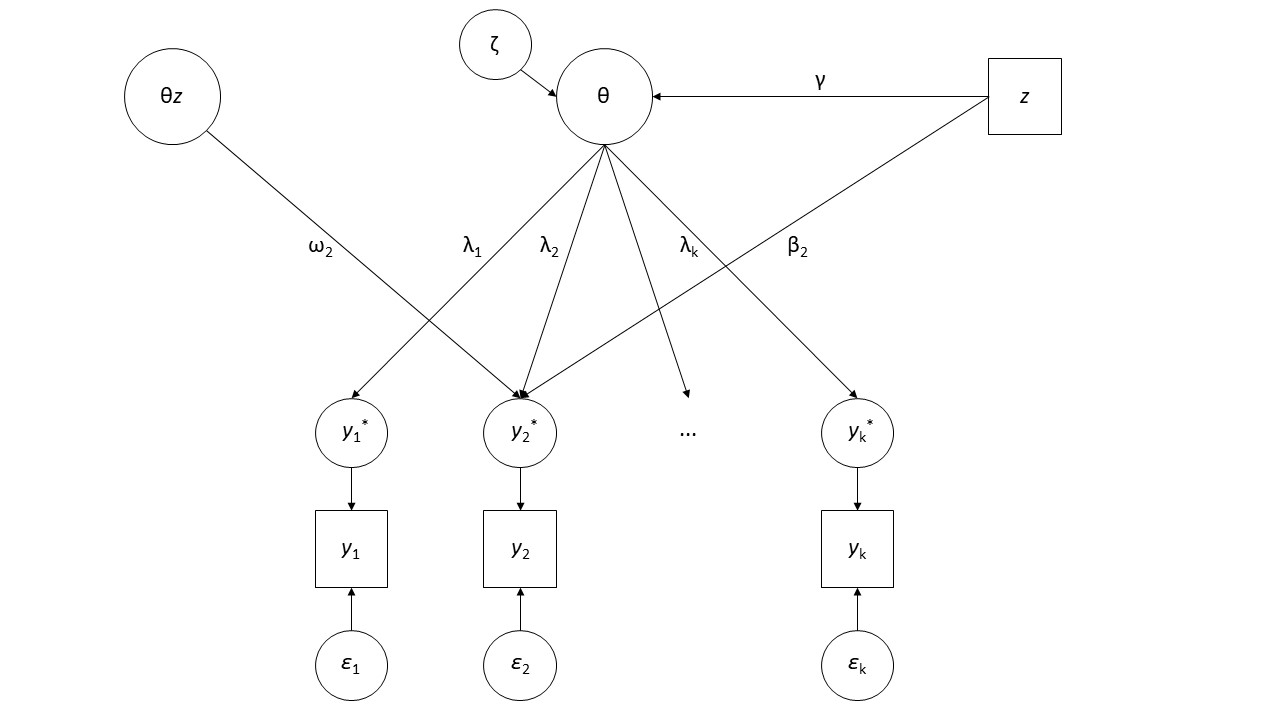
\includegraphics[scale = 0.45]{MIMIC_model.jpg}
    \caption{Schematic illustration of the MIMIC model for detecting uniform and nonuniform DIF for item 2.}
    \label{fig:mimicmodel}
\end{figure}

There are multiple strategies to use the MIMIC model and it is out of the scope of this paper to discuss them all (see \citet{lee2018methodological} for further reading). The constrained-baseline strategy tests one item for DIF at a time, while the other items are assumed to be DIF-free. First, a baseline model is fitted to the data without direct effects. Then, the fit of the baseline model is evaluated against $i$ models (where $i$ is the number of items) that specify a direct effect between one item and the grouping variable, while controlling for group differences by regressing the construct on the grouping variable, and an interaction term between the construct and the grouping variable \citep{lee2018methodological}. Figure \ref{fig:mimicmodel} displays an example of this item model, where the second item is tested for DIF. The MIMIC model for item $i$ can be written as:

\begin{equation} \label{eq:mimic_oneitem}
    y_i^* = \lambda_i\theta + \beta_i z + \omega_i\theta z + \varepsilon_i,
\end{equation}

where $y_i^*$ is the latent ability underlying the observed item response for item $i$, $\lambda_i$ is the factor loading for item $i$ (the item discrimination parameter in IRT models), $\theta$ is the latent ability that follows a normal distribution, $z$ is the dummy-coded grouping variable, $\beta_i$ is the uniform DIF effect for item $i$, $\omega_i$ is the nonuniform DIF effect for item $i$, and $\varepsilon_i$ is the random error for item $i$ \citep{bulut2017detecting}. Uniform and nonuniform DIF for item $i$ are present when $\beta_i \neq 0$ and $\omega_i \neq 0$, respectively. 

\subsection{Propensity Score Matching} \label{sec:psm}

PSM originated in the context of non-randomized experiments as a proxy for random assignment and constructs comparable groups by equating sampling groups on propensity scores based on background characteristics \citep{rosenbaum1983central}. Three steps constitute the matching process: selecting covariates (\ref{sec:cov}), estimating propensity scores and matching (\ref{sec:est_psm}), and evaluating covariate balance (\ref{sec:balance}). 

\subsubsection{Selecting covariates} \label{sec:select_cov}

The first step in PSM is selecting covariates to match the groups on. Although there is some discourse regarding this topic, the consensus is that including covariates that are related to both the construct and the grouping variable generates the best performance \citep{stuart2010matching}. 

\subsubsection{Estimating propensity scores and matching} \label{sec:est_psm}

After selecting covariates for matching, propensity scores can be estimated. A propensity score is the conditional probability of an individual belonging to the focal group given the selected covariates and can be expressed as:

\begin{equation} \label{eq:ps}
    e(\mathbf{X_i}) = P(Z_i = 1 | \mathbf{X_i}),
\end{equation}

where $e(\mathbf{X_i})$ is the propensity score for individual $i$, $Z_i$ is the indicator of the grouping variable of individual $i$, $Z_i = 1$ denotes the individuals $i$ belonging to the focal group and $\mathbf{X_i}$ is the vector of scores on the selected covariates for individual $i$ \citep{rosenbaum1983central}. Propensity scores are usually estimated through logistic regression:

\begin{equation} \label{eq:logreg}
    P(Z_i = 1 | \mathbf{X_i}) = \frac{e^{\beta_0 + \mathbf{\beta(x_i)}}}{1 + e^{\beta_0 + \mathbf{\beta(x_i)}}}, 
\end{equation}

where $\beta_0$ is the intercept and $\mathbf{\beta(x_i)}$ is a vector of coefficients for the included covariates \citep{rosenbaum1983central}. 

The estimated propensity scores are matched to adjust for group differences. There are multiple ways to do this and it is advised to apply multiple methods as their performance differs based on the data \citep{liu2016investigating}. Matching methods can broadly be divided into greedy and optimal matching. 

\paragraph{Greedy matching} Greedy matching methods do not optimize a criterion, which means that units are matched once, without accounting for how other units will be or have been matched. For example, in Nearest Neighbor Matching (NNM), a random unit in the focal group is selected and paired with the closest unit in the reference group, after which the algorithm turns to the next focal unit and repeats this process until all focal units are paired \citep{stuart2010matching, liu2016investigating}. 

\paragraph{Optimal matching} Contrary to greedy matching, matches can be redone in optimal matching until a specified criterion is optimized. The most common optimal matching methods are optimal pair (OPM) and optimal full matching (OFM). OPM matches in pairs and discards the remaining unmatched units, while OFM allows one focal unit to be matched to multiple reference units (one-to-many) or multiple focal units to one reference unit (many-to-one) \citep{stuart2010matching, liu2016investigating}. 

\subsubsection{Evaluating the covariate balance} \label{sec:balance}

After matching, the performance of the different methods is evaluated by examining the distance within the matched pairs and the balance of the matched groups \citep{gu1993comparison}. The distance within pairs implies that the values of the matched units on covariate $X$ should be as close as possible. The difference between the propensity scores of the matched focal and reference units is a measure of this distance \citep{stuart2010matching}. 

The matched groups are balanced when the distribution of covariate $X$ in the focal group resembles that of the reference group in the matched subsample. Balance can be assessed visually, by comparing histograms and density plots of the groups before and after matching, or by computing measures that quantify the difference between the distributions. Examples of such statistics are standardized mean differences, which should be close to 0, or variance ratios, which should be close to 1 \citep{chen2020propensity}. 

\subsection{Propensity Score Matching in Educational Assessment}

Relatively few studies have applied PSM to education assessment data. \citet{seo2015comparability} studied mode comparability in the Michigan Educational Assessment Program. They found the modes to be comparable after matching students on gender, ethnicity, special education, English proficiency, economic disadvantage, and mathematics and readings scores for students and schools. \citet{puhan2005evaluating} reached a similar conclusion when they analyzed mode comparability in a teacher certification test by matching teachers on gender, language, test repeater status, race, GPA, and education level.

Apart from mode effects, other causes of DIF have also been studied using PSM. \citet{wu2006using} looked at the effect of Extra Lesson Hours After School (ELHAS) on DIF between Taiwanese and U.S. students in TIMSS. They found that matching students on ELHAS resulted in a reduction in the number of items displaying DIF. Further, \citet{joldersma2010application} examined DIF due to language in a Language Arts Literacy assessment that was translated from English to Spanish. After matching students on gender, economic status, and total test score, they found that item bias was eliminated in both versions of the test. Additionally, \citet{lee2014effect} studied gender DIF in an English reading test administered to South Korean college students. They found that matching students on interest in education resulted in a reduction in the number of items displaying DIF. Moreover, \citet{arikan2018propensity} used the PISA 2012 math items to investigate the effect of different PSM methods on DIF results and the achievement differences among Indonesian, Turkish, Australian, and Dutch students. They matched students on gender, opportunity to learn, and the index of economic, social and cultural status, and found that PSM reduced the number of items flagged for DIF and also diminished country differences.  

\section{Method} \label{Method}

\subsection{Data} \label{sec:data}

The publicly available \href{https://www.oecd.org/pisa/data/2018database/}{PISA data of 2018} were used in this study. PISA is an international assessment study that takes place every three years, measuring 15-year-old students' skills and knowledge in reading, mathematics and science. Approximately 710,000 students completed the test in 2018, representing over 31 million students in 79 participating countries and economies \citep{PISA2018assessment}. PISA was computer-administered in the majority of the participating countries. However, for students in nine countries (Argentina, Jordan, Lebanon, Moldova, North Macedonia, Romania, Saudi Arabia, Ukraine and Vietnam), the test was paper-administered. Figure \ref{fig:landenkaart} presents a map of the world that shows which countries participated in PISA and the mode of test administration. 

As PISA aims to measure a broad scope of knowledge in a limited amount of testing time, an integrated test design is used in which students only make a subset of the total number of items through multiple test versions, called booklets. Each booklet covers two domains and contains four clusters of items, with each cluster covering one domain and taking thirty minutes to complete. In addition to the test, students complete a 35-minute questionnaire in which information on the students themselves, their homes, and their school and learning experiences is gathered. As different booklets are used for PBA and CBA, booklets 1 and 13 were selected for this study. These were regular booklets with an identical fixed unit order for both modes. Moreover, they were administered to a large number of students, specifically 2303 and 20,288 students from 9 and 70 countries, for PBA and CBA respectively. 

\begin{figure} [!ht]
    \centering
    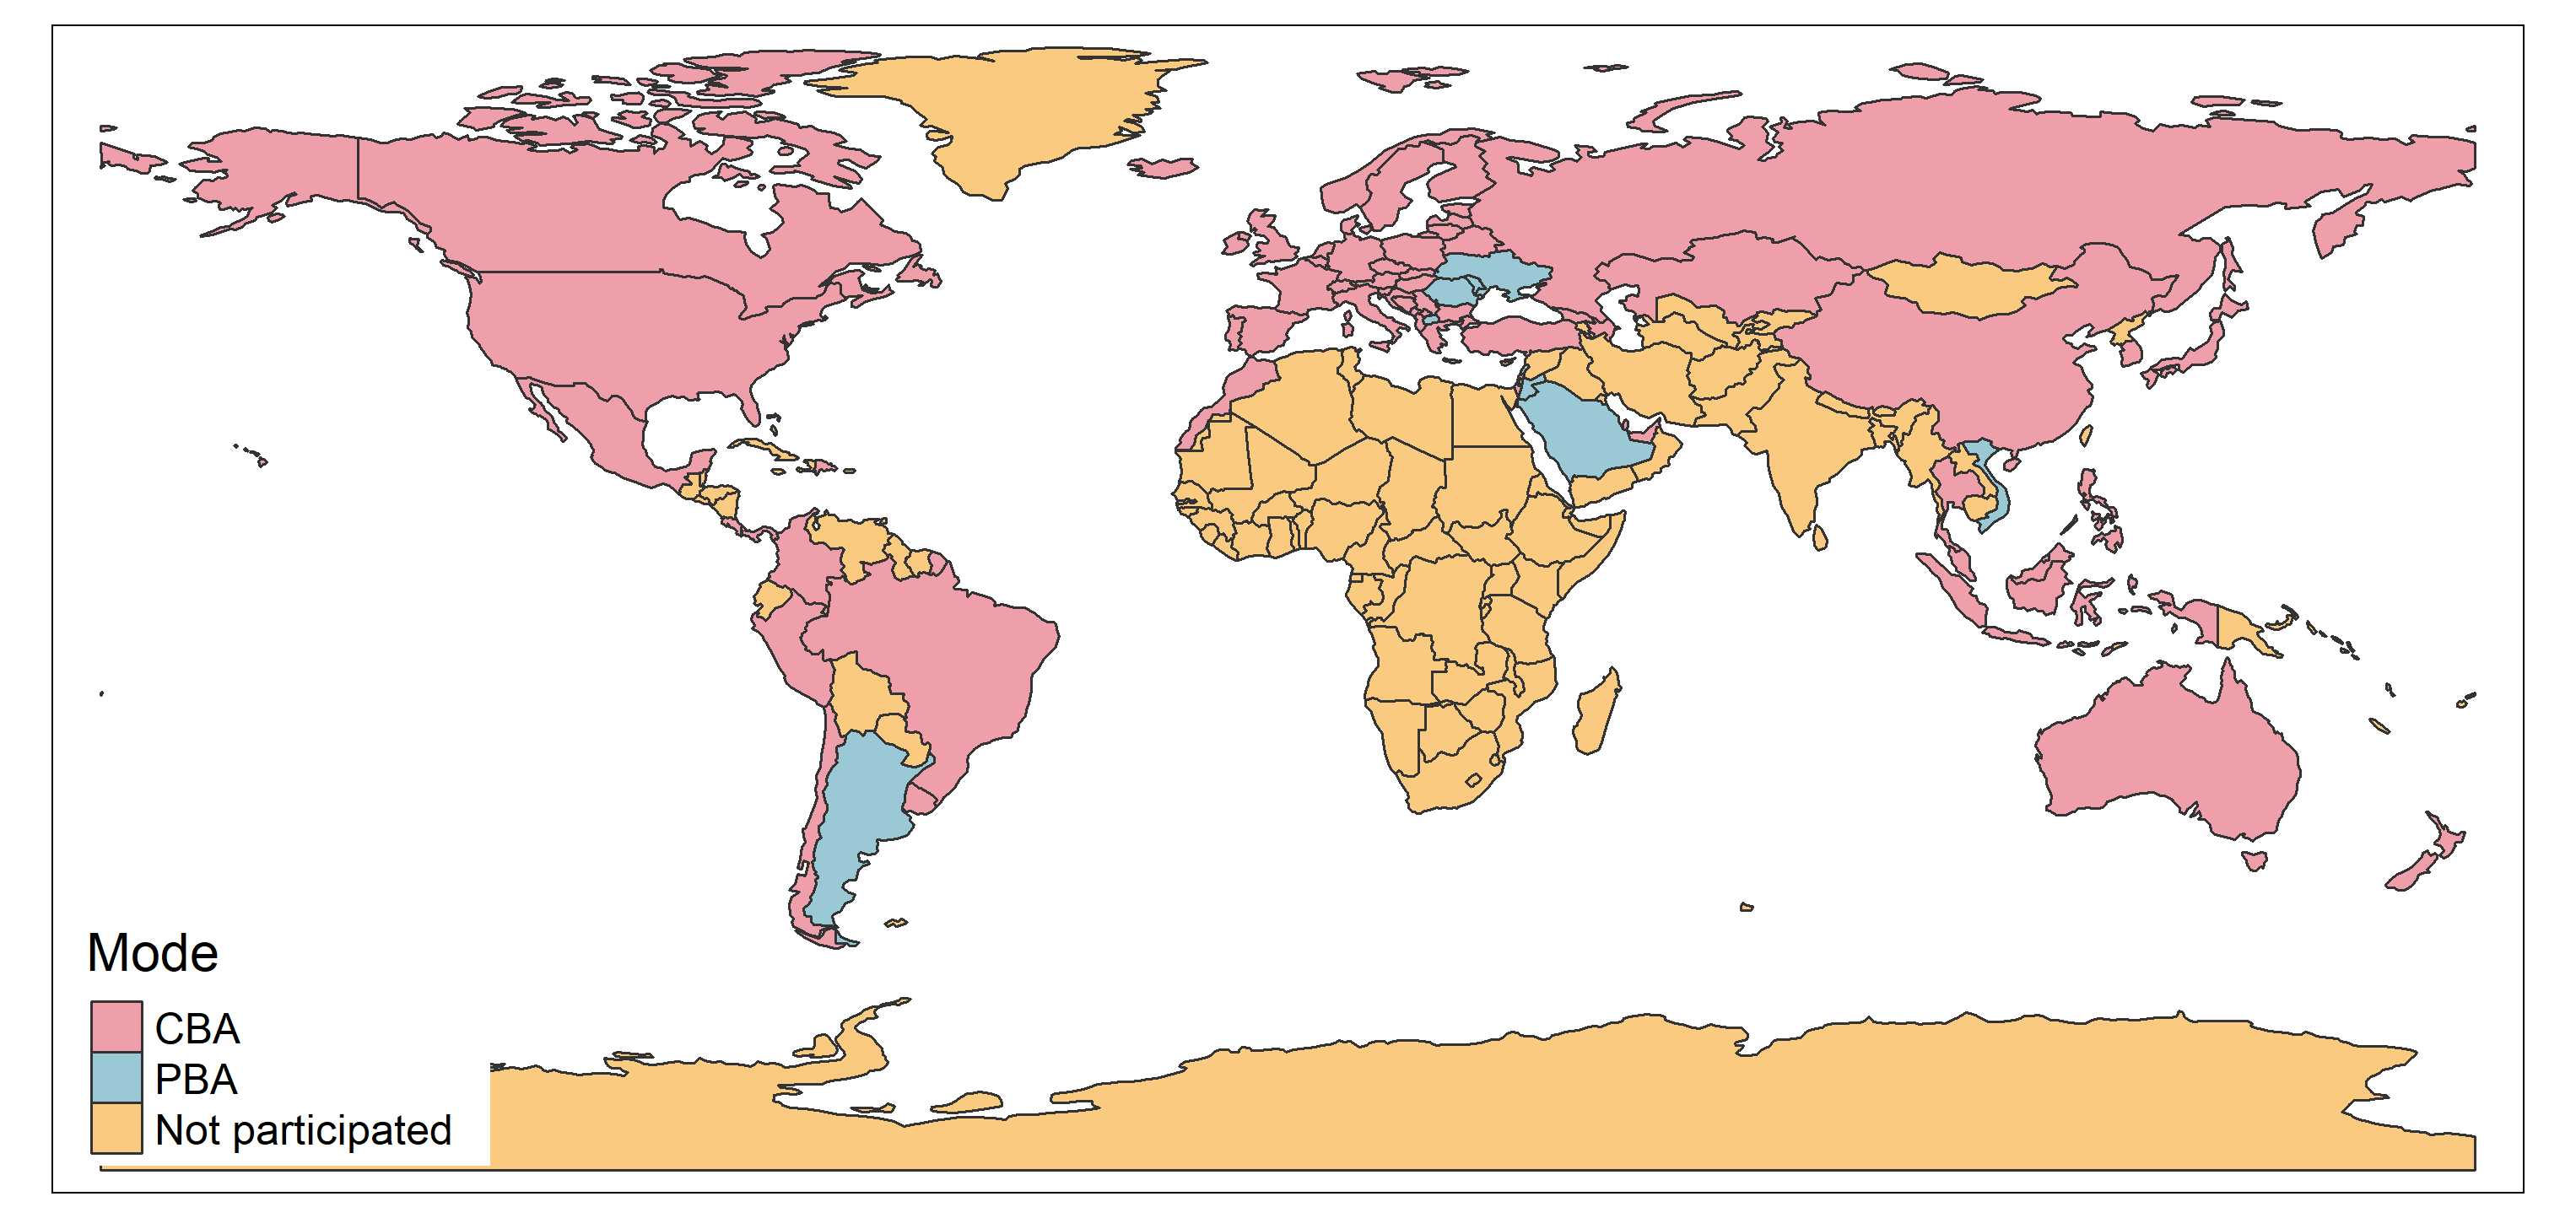
\includegraphics[scale = 0.58]{mode_map.png}
    \caption{Map of the world showing the participating countries in PISA 2018 and whether the students made the test on a computer (CBA) or on paper (PBA).}
    \label{fig:landenkaart}
\end{figure}

\subsection{Instruments}

\paragraph{Science items}

Booklets 1 and 13 consist of the first two out of a total of six science clusters that cover 38 of the 115 available science items. Out of the 38 items, three were scored polytomously. All other items were dichotomously scored. Moreover, 13 items were open responses and the remaining 25 items were either simple or complex multiple-choice items. Additional information on the items can be found in Annex A of the \href{https://www.oecd.org/pisa/data/pisa2018technicalreport/}{PISA 2018 technical report}.

\paragraph{Covariates} \label{sec:cov} Apart from test data, PISA collects an abundance of background information, which is stored in a questionnaire dataset. The index of economic, social and cultural status (ESCS) is probably the most important variable. This variable is constructed by PISA as a composite measure, including highest parental occupation, an index representing parental education, and an index of household possessions which functioned as a proxy for family income. Apart from ESCS, the other covariates included the effort the students have put in the PISA test, the effort they would have put in a graded test, the number of class periods in science, and gender.

\subsection{Data Analysis}

\subsubsection{Pre-processing} \label{sec:pre-processing}
First, the items of the first two science clusters in the selected booklets were extracted from the test data, as well as the country and student ID within the country. The items in the PBA and CBA booklets were combined and a dummy variable was constructed to indicate the mode of administration. Similarly, the questionnaire data was filtered, such that only the data of the selected booklets remained. Next, cases of unit nonresponse were deleted and item nonresponse cases were replaced with a 0 when the student left the question open.

The item responses were recoded into numeric variables where 0 equaled no credit and 1 equaled full credit for binary items and partial credit for polytomous items, for which a 2 equaled full credit. One item (\textit{DS438Q03C}) was polytomously scored, while the second and third categories corresponded to full credit. This item was recoded such that the categories were collapsed into a single 1 full credit score. 

\subsubsection{Detecting DIF}

After pre-processing, the first step was to detect DIF using the MIMIC model under the constrained-baseline strategy as described in Section \ref{sec:mimic}. The students' science ability was the construct of interest and the dummy-coded mode-indicator served as the grouping variable. We evaluated the presence of DIF by comparing a model for each item against the baseline model with a $\chi^2$-difference test. The item was subject to DIF if the item model fitted significantly better than the baseline model. Then, the significance of the $\beta_i$ and $\omega_i$ parameters determined the DIF-type, respectively corresponding to uniform and nonuniform DIF. Herein, Bonferroni's correction criterion was applied, such that $p < 0.001$ was considered statistically significant.

\subsubsection{Applying Propensity Score Matching}

Once DIF was detected, the second step was applying PSM. Section \ref{sec:cov} discussed the selected covariates. Propensity scores were estimated using logistic regression and matched using three methods: NNM, OPM and OFM (discussed in Section \ref{sec:est_psm}), which resulted in three matched subsamples. Subsequently, the performance of the methods was evaluated by visually comparing histograms and density plots before and after matching, as well as examining standardized mean differences and variance ratios for each covariate. Then, the MIMIC model as described above was applied again with the matched subsamples as input data to investigate how matching affected the number of items displaying DIF.

\subsubsection{Constructing Country League Tables}

The last step was to construct country league tables, wherein we followed PISA's methodology \citep{OECD2018}. The unidimensional IRT model for dichotomous responses and generalized partial credit model for polytomous responses were fitted to each of the three matched subsamples to estimate a set of item parameters for each matching method (three sets in total). Returning to the full sample, these item parameters were used to draw ten plausible values for each student per Rubin's rules. This resulted in three sets of ten plausible values for each student in the full sample. The plausible values were weighted to account for the survey design and pooled into an estimate of the science ability for each country. Ordering them for high to low resulted in a country league table for each matching method, which were compared to the table originally published by PISA for differences to inspect how the matching methods affected the ranking order.

\subsubsection{Software} 
Due to the file size, the initial extraction of the test and questionnaire data corresponding to the selected booklets was done in SPSS \citep{spss}. All other analyses were performed in RStudio \citep{Rstudio2020}, using the packages ``lavaan'' \citep{lavaan2012}, ``MatchIt'' \citep{MatchIt2011} and ``cobalt'' \citep{greifer2020cobalt}. Accompanying syntax and code are available through \href{https://github.com/agjtimmers/CitoThesis}{Github}. 

\section{Results}

\subsection{Example Table}

\begin{center}
\begin{table}
\renewcommand{\arraystretch}{2}
\begin{tabular*}{1\textwidth}{@{\extracolsep{\fill}} l c c c c c c}
    \hline
    \hline
    & \multicolumn{3}{c}{Before matching} & \multicolumn{3}{c}{Nearest Neighbor Matching} \\
    \midrule
    Covariate & Computer & Paper & Difference & Computer & Paper & Difference \\
    \hline
    ESCS & 0 & 0 & 0 & 0 & 0 & 0 \\
    Effort PISA & 0 & 0 & 0 & 0 & 0 & 0 \\
    Effort graded & 0 & 0 & 0 & 0 & 0 & 0 \\
    Science classes & 0 & 0 & 0 & 0 & 0 & 0 \\
    Gender & 0 & 0 & 0 & 0 & 0 & 0 \\
    \hline
\end{tabular*}

\begin{tabular*}{1\textwidth}{@{\extracolsep{\fill}} l c c c c c c}
    & \multicolumn{3}{c}{Optimal Pair Matching} & \multicolumn{3}{c}{Optimal Full Matching} \\
    \midrule
    Covariate & Computer & Paper & Difference & Computer & Paper & Difference \\
    \hline
    ESCS & 0 & 0 & 0 & 0 & 0 & 0 \\
    Effort PISA & 0 & 0 & 0 & 0 & 0 & 0 \\
    Effort graded & 0 & 0 & 0 & 0 & 0 & 0 \\
    Science classes & 0 & 0 & 0 & 0 & 0 & 0 \\
    Gender & 0 & 0 & 0 & 0 & 0 & 0 \\
    \hline
    \hline
\end{tabular*}
\caption{Standardized means of matching variables for computer and paper students before and after matching, and their difference.}
\end{table}
\end{center}

\newpage
\printbibliography
\end{document}
